\chapter{Evaluation Chapter Attachments}
\label{ap:evaluation-instructions}

\section{Time Analysis}

\medskip
\noindent
{\it R Instructions}
\begin{verbatim}
exp1.dat = read.table(file="/home/me/r_input.dat", header = T)
attach(exp1.dat)

replica = factor(replica.)
student = factor(student.)
program = factor(program.)
lock = factor(lock.)

# Calculate average time for each lock

aggregate(time, by=list(lock), FUN=mean)

# Plot the box plot graphic using the response variable
# associated with the techniques

plot(time~lock,col="gray",xlab="Lock",ylab="Time(seconds)")

# Through the following command we adjust the effect model
# that will serve as basis for posterior analysis.

anova.ql<-aov(time~replica+student:replica+program+lock)

library(MASS)
bc <- boxcox(anova.ql,lambda = seq(-3, 5, 1/10))

# Calculate lambda for boxcox transformation

lambda <- bc$x[which.max(bc$y)] 

# If lambda is not approximately 1, run the next command
# with [a] replaced by lambda's value found previously:
# anova.ql<-aov(time**[a]~replica+student:replica+program+lock)
# Then confirm that the new curve maximum is close to 1: 
# bc <- boxcox(anova.ql,lambda = seq(-3, 5, 1/10))

TukeyNADD.QL.REP<-function(objeto1)
{
y1<-NULL
y2<-NULL
y1<- fitted(objeto1)
y2<- y1^2
objeto2<- aov(y2 ~ objeto1[13]$model[,2] +
objeto1[13]$model[,3]:objeto1[13]$model[,2]
+ objeto1[13]$model[,4]+ objeto1[13]$model[,5])
ynew <- resid(objeto1)
xnew <- resid(objeto2)
objeto3 <- lm(ynew ~ xnew)
M <- anova(objeto3)
MSN <- M[1,3]
MSErr <- M[2,2]/(objeto1[8]$df.residual-1)

F0 <- MSN/MSErr
p.val <- 1 - pf(F0, 1,objeto1[8]$df.residual-1)
p.val
}

# Return p-value for Tukey additivity test
TukeyNADD.QL.REP(anova.ql)

# Run ANOVA to see what factor was most significant
anova(anova.ql)
\end{verbatim}

\medskip
\noindent
{\it First Experiment Input}
\begin{verbatim}
replica, student, program, lock, time
1, 1, p1, A, 4967
1, 1, p2, B, 5413
1, 2, p1, B, 5400
1, 2, p2, A, 5320
2, 3, p1, A, 2340
2, 3, p2, B, 5290
2, 4, p1, B, 5400
2, 4, p2, A, 4210
3, 5, p1, A, 5400
3, 5, p2, B, 5360
3, 6, p1, B, 3600
3, 6, p2, A, 2406
4, 7, p1, A, 3290
4, 7, p2, B, 5370
4, 8, p1, B, 5070
4, 8, p2, A, 5260
5, 9, p1, A, 3000
5, 9, p2, B, 5315
5, 10, p1, B, 5400
5, 10, p2, A, 3641
6, 11, p1, A, 3424
6, 11, p2, B, 5356
6, 12, p1, B, 5400
6, 12, p2, A, 4788
7, 13, p1, A, 5400
7, 13, p2, B, 5400
7, 14, p1, B, 5400
7, 14, p2, A, 5160
8, 15, p1, A, 5280
8, 15, p2, B, 5160
8, 16, p1, B, 4490
8, 16, p2, A, 4017
9, 17, p1, A, 2700
9, 17, p2, B, 5306
9, 18, p1, B, 5090
9, 18, p2, A, 4450
10, 19, p1, A, 4271
10, 19, p2, B, 5569
10, 20, p1, B, 3377
10, 20, p2, A, 4473
11, 21, p1, A, 5160
11, 21, p2, B, 5430
11, 22, p1, B, 4174
11, 22, p2, A, 4886
12, 23, p1, A, 2027
12, 23, p2, B, 4271
12, 24, p1, B, 5400
12, 24, p2, A, 3804
13, 25, p1, A, 4996
13, 25, p2, B, 5367
13, 26, p1, B, 5310
13, 26, p2, A, 5390
14, 27, p1, A, 3860
14, 27, p2, B, 5119
14, 28, p1, B, 4705
14, 28, p2, A, 4535
15, 29, p1, A, 2593
15, 29, p2, B, 5279
15, 30, p1, B, 5250
15, 30, p2, A, 4246
\end{verbatim}

\medskip
\noindent
{\it Second Experiment Input}
\begin{verbatim}
replica, student, program, lock, time
1, 1, p1, A, 1757
1, 1, p2, B, 2404
1, 2, p1, B, 1777
1, 2, p2, A, 1716
2, 3, p1, A, 1342
2, 3, p2, B, 2552
2, 4, p1, B, 2597
2, 4, p2, A, 1238
3, 5, p1, A, 1572
3, 5, p2, B, 2248
3, 6, p1, B, 3168
3, 6, p2, A, 2460
4, 7, p1, A, 1822
4, 7, p2, B, 2455
4, 8, p1, B, 2486
4, 8, p2, A, 2434
5, 9, p1, A, 3503
5, 9, p2, B, 3600
5, 10, p1, B, 2454
5, 10, p2, A, 1753
6, 11, p1, A, 1830
6, 11, p2, B, 3300
6, 12, p1, B, 2880
6, 12, p2, A, 890
7, 13, p1, A, 648
7, 13, p2, B, 940
7, 14, p1, B, 2247
7, 14, p2, A, 1363
\end{verbatim}

\section{Accuracy Analysis}

\medskip
\noindent
{\it R Instructions}
\begin{verbatim}
# Use TSV export feature on each set of results:
# [1] https://goo.gl/EPxmEa (first experiment)
# [2] https://goo.gl/rsWPwi (second experiment)
# Run http://pastebin.com/rSBjTiYj on each

fisher.test(rbind(c(29,2),c(16,15)), alternative="two.sided")
fisher.test(rbind(c(13,1),c(10,4)), alternative="two.sided")
\end{verbatim}

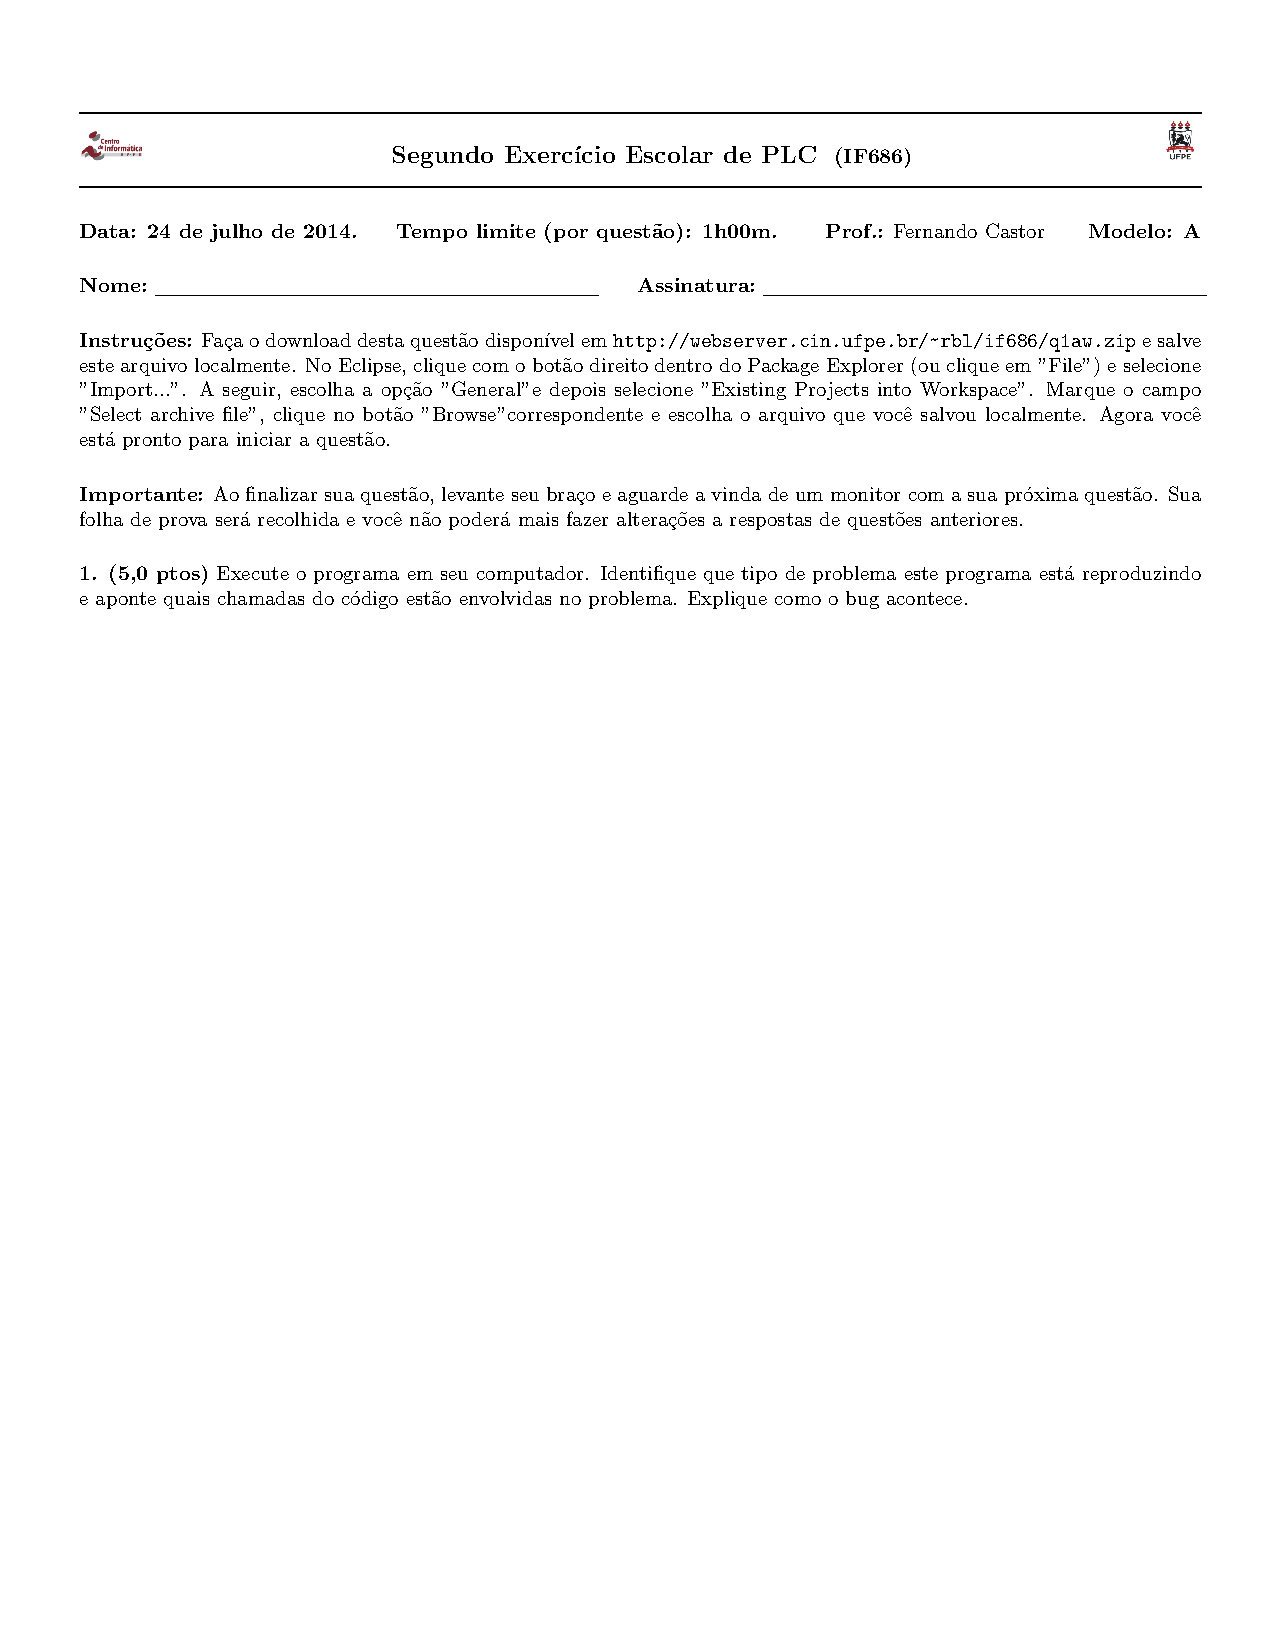
\includepdf[scale=0.8,pages=1,pagecommand=\section{Experiment First Assignment}]{appendix/sample-question.pdf}

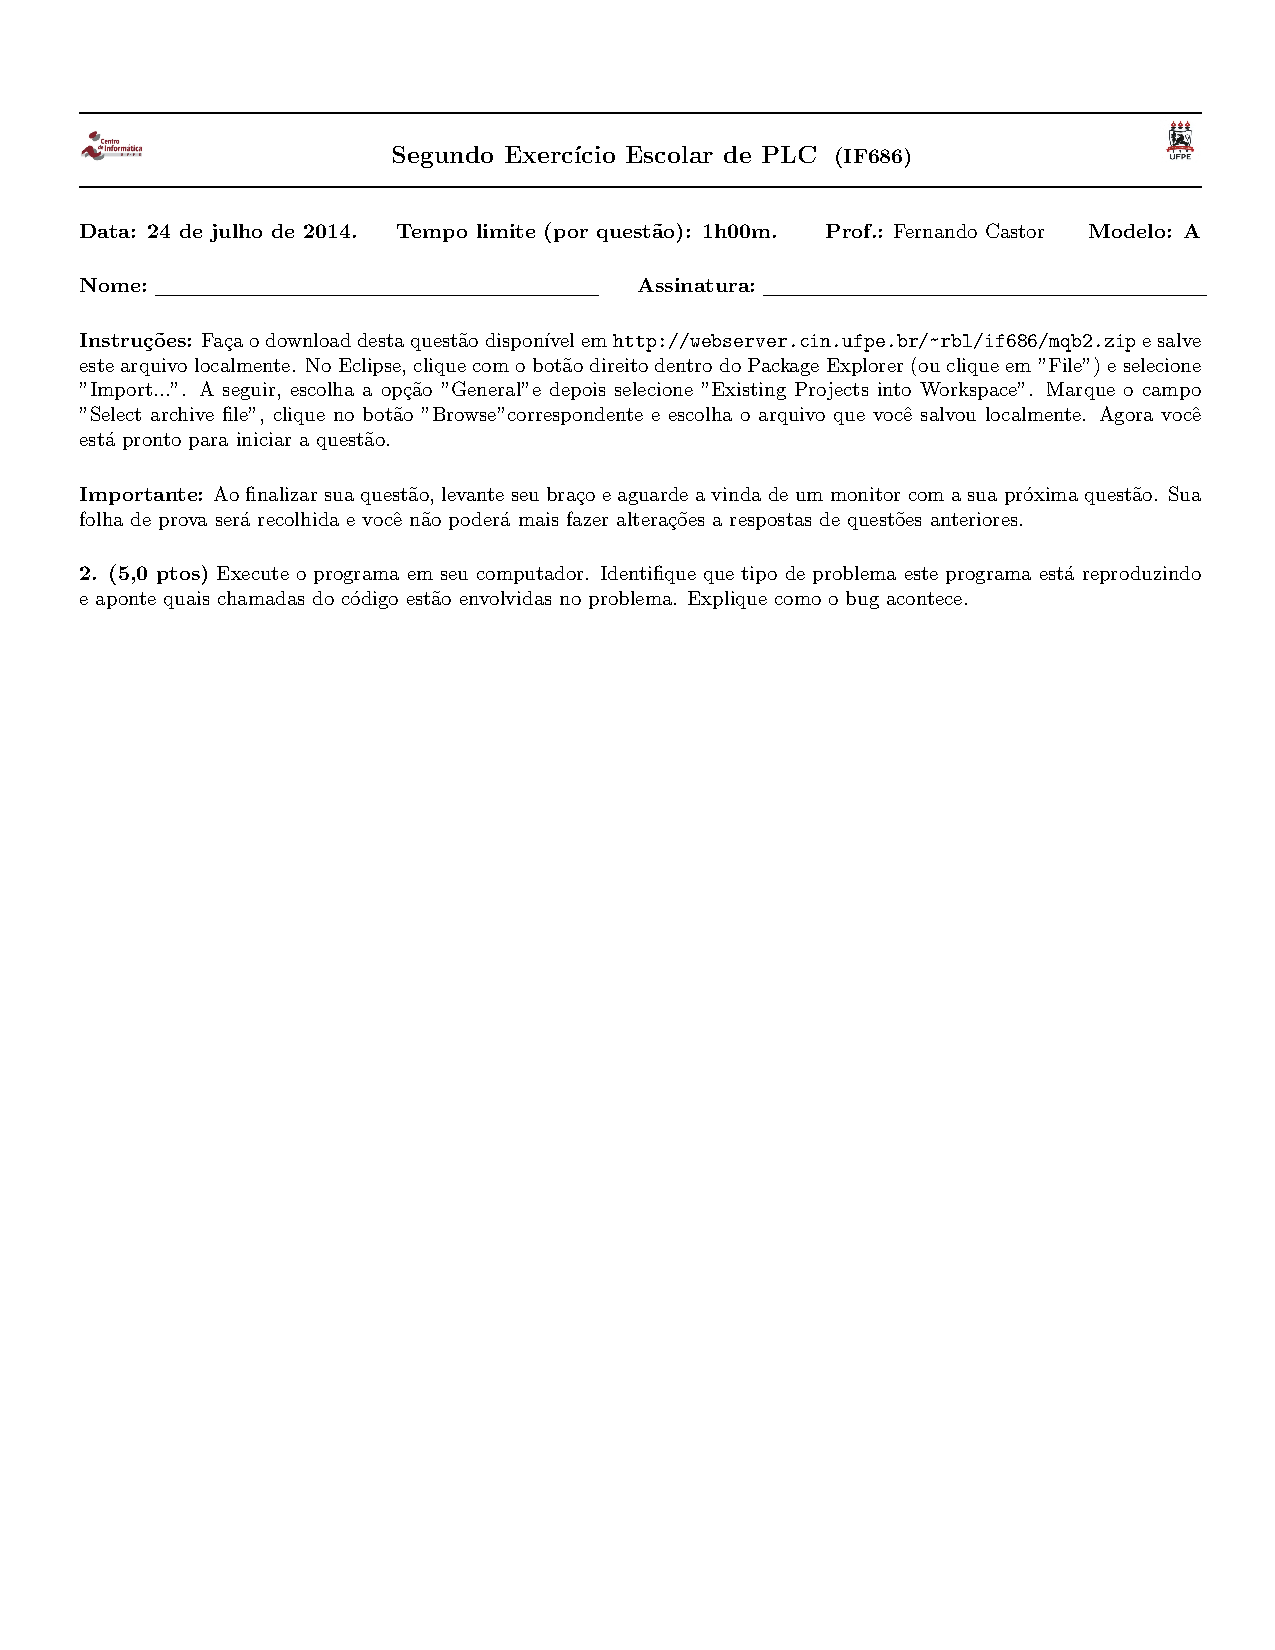
\includepdf[scale=0.8,pages=1,pagecommand=\section{Experiment Second Assignment}]{appendix/sample-question-2.pdf}

